\documentclass[10pt,conference]{IEEEtran}
\IEEEoverridecommandlockouts
\usepackage{cite}
\usepackage{amsmath,amssymb,amsfonts}
\usepackage{graphicx}
\usepackage{textcomp}
\usepackage{xcolor}
\usepackage{url}
\usepackage[hidelinks]{hyperref}
\usepackage{booktabs}
\setlength{\textfloatsep}{5pt plus 2pt minus 2pt}
\setlength{\floatsep}{4pt plus 2pt minus 2pt}
\setlength{\intextsep}{4pt plus 2pt minus 2pt}
\setlength{\abovecaptionskip}{3pt}
\setlength{\belowcaptionskip}{0pt}
\begin{document}

\title{Hardware-Aware Quantum Bayesian Learner Compression:\\ Linking Human Belief Updating to NISQ Circuit Complexity}

\author{
\IEEEauthorblockN{Mohammad Zoraiz}
\IEEEauthorblockA{
\textit{Pratt School of Engineering, Duke University} \\
Electrical Engineering, Physics, and Computer Science, Durham, NC, USA \\
mz248@duke.edu}
}

\maketitle

\begin{abstract}
We connect quantum models of cognition with the constraints of near-term quantum hardware. A
small \emph{quantum Bayesian learner}---a belief state on a two-qubit register, a prior, and a
stimulus-dependent evidence channel---learns a similarity-structured categorization task, with
the posterior category read out by measurement. Making the learner a hardware-efficient
variational circuit, we add a hardware-aware penalty equal to the real post-transpile two-qubit
gate count on IBM's \texttt{FakeManila} backend and compress it by greedy structured pruning of
individual Heisenberg interaction terms. Across three difficulty levels and five seeds, the
accuracy--complexity frontier reveals a sharp \emph{capacity boundary}: structured compression
is essentially free---and on the hardest task beneficial---yet removing all entanglers collapses
the learner to chance. Learned masks beat random masks at every matched budget. On a physical
IBM device (\texttt{ibm\_fez}), the full circuit collapses to near chance while the compressed
circuit stays accurate: on real NISQ hardware, hardware-aware compression is not merely
economical but necessary.
\end{abstract}

\begin{IEEEkeywords}
Quantum cognition, Bayesian learning, variational quantum circuits, hardware-efficient ansatz,
NISQ devices, circuit compression.
\end{IEEEkeywords}

\section{Introduction}
Bayesian models cast human learning as \emph{belief updating}: a prior over hypotheses revised
by evidence \cite{b1}. \emph{Quantum cognition} represents belief states in Hilbert space---as
density operators---and updates them with the mathematics of quantum channels, capturing
interference and order effects \cite{b3}. In parallel, noisy intermediate-scale quantum (NISQ)
devices \cite{b7} have made variational quantum algorithms the dominant near-term paradigm
\cite{b6}, built from hardware-efficient ans\"atze of single-qubit rotations and native
two-qubit entanglers \cite{b4,b5}. Because two-qubit gates dominate the NISQ error budget
\cite{b7,b10}, reducing their number without destroying task performance is a central
engineering objective.

We join these threads. The belief is a state on a two-qubit register, the evidence update is a
stimulus-conditioned channel, and training is on a similarity-structured categorization task
\cite{b19}; the update circuit is a Heisenberg-type hardware-efficient ansatz, and a
hardware-aware loss penalizes the two-qubit gates remaining after transpilation. The guiding
question is concrete: \emph{how much of the circuit can be removed before the learner can no
longer represent the task?} Our contributions are (1)~a compact quantum Bayesian learner in the
density-operator/channel language, exactly simulated and analytically differentiable; (2)~a
hardware-aware cost equal to the real post-transpile two-qubit count on \texttt{FakeManila},
resolved per $R_{XX}/R_{YY}/R_{ZZ}$ term; (3)~accuracy--complexity frontiers locating a
\emph{capacity boundary}; (4)~a learned-versus-random ablation; and (5)~validation on a physical
IBM device.

\section{Methods}
\textbf{Belief states and evidence channels.} The belief about a stimulus is a state $\rho$ on
$n{=}2$ qubits. A prior $\rho_0$ is updated by a completely-positive trace-preserving channel
conditioned on the stimulus $x$,
$\mathcal{E}_x(\rho)=\sum_k E_{x,k}\,\rho\,E_{x,k}^{\dagger}$, with the posterior read out by
measurement \cite{b3}. A fast \emph{pure-state} model takes
$\rho_0=\lvert0\rangle\!\langle0\rvert^{\otimes n}$ with a unitary evidence channel; a literal
\emph{mixed-state} model starts from the maximally mixed prior $\mathbb{I}/2^n$ and applies a
non-unital evidence channel---a stimulus-dependent L\"uders/POVM filter with Bayesian trace
renormalization plus amplitude damping---so the belief is a bona fide mixed state (verified PSD,
unit-trace, purity${<}1$). Both are exactly simulated and analytically differentiable, and the
mixed model reduces bit-for-bit to the pure one when the channel is off.

\textbf{Ansatz and hardware-aware cost.} Each of $D{=}4$ layers applies single-qubit $R_X,R_Z$
rotations and a Heisenberg entangler
$U_{ij}=\exp[-i(\alpha X_iX_j+\beta Y_iY_j+\gamma Z_iZ_j)]$ realized as native
$R_{XX},R_{YY},R_{ZZ}$, interleaved with data re-uploading \cite{b4,b5}. A per-term binary mask
$m_{\ell,p}\in\{0,1\}$ selects each interaction term (12 maskable terms; $R_{PP}(0)=\mathbb{I}$
when off), a small instance of quantum architecture search \cite{b16}. The cost $N_{2q}(m)$ is
the real number of two-qubit gates surviving transpilation to \texttt{FakeManila} (including
SWAPs), computed via Qiskit's transpiler \cite{b24}; the full circuit gives $N_{2q}{=}24$. The
objective is $L(\theta,m)=\frac1N\sum_k \mathrm{BCE}(y_k,\hat y_k)+\lambda N_{2q}(m)$. The
readout uses only \emph{single-qubit} Pauli expectations
$(\langle Z_0\rangle,\langle Z_1\rangle,\langle X_0\rangle,\langle X_1\rangle)$ through a
trainable head $\hat y=\sigma(w\cdot v+b)$; this makes entanglement the \emph{only} carrier of
feature interaction, so $N_{2q}$ meaningfully bounds the learner's capacity.

\textbf{Compression and task.} Parameters are trained by Adam with exact JAX autodiff through
the belief-state simulator (verified bit-for-bit against Qiskit). \emph{Greedy structured
pruning} repeatedly removes the term whose removal least increases training cross-entropy,
warm-start retraining after each step, tracing the accuracy--$N_{2q}$ frontier from 24 to 0. The
task is a checkerboard categorization
$y=(\lfloor f x_0\rfloor+\lfloor f x_1\rfloor)\bmod 2$ on $[0,1]^2$ \cite{b19}, with a difficulty
knob $f{=}2,3,4$ (easy/medium/hard); 200 balanced stimuli are split $70/30$ (chance $0.5$).

\section{Results}
\textbf{Capacity boundary.} The learner is well above chance at all nonzero budgets (easy/medium
$\approx0.95$--$0.97$, hard $\approx0.87$--$0.93$) and the frontier is nearly flat, so most
entangling structure is redundant; at $N_{2q}{=}0$ every difficulty collapses toward chance
($0.52$/$0.64$/$0.49$). Some entanglement is thus necessary but far less than the full circuit.
On the hard task accuracy \emph{peaks} at intermediate cost ($0.927$ at $N_{2q}{=}6$) and is
lower for the full circuit ($0.873$ at $N_{2q}{=}24$): moderate compression acts as a
capacity-control regularizer.

\textbf{Structure beats count.} At matched budgets, greedy (learned) masks beat random masks of
identical sparsity at \emph{every} budget by $\sim$6--12 points (Table~\ref{tab:ablation});
per seed, the learned mask wins $49$ of $55$ paired comparisons, mean advantage $+0.083$,
one-sided Wilcoxon $p<10^{-7}$. \emph{Which} entanglers are kept matters, not only how many.

\textbf{Validation on hardware.} On a physical IBM processor (\texttt{ibm\_fez}, a $156$-qubit
Heron device, hard task), the on-device frontier \emph{reverses} the simulated picture
(Fig.~\ref{fig:hw}): accuracy falls monotonically with $N_{2q}$---$0.81$ at $N_{2q}{=}2,6$,
$0.75$ at $12$, and $0.56$ (near chance) at $18,24$. A denser endpoint run confirms the full
circuit at $0.60$ (simulation $0.95$) versus the compressed circuit at $0.83$ (simulation
$0.93$). On real NISQ hardware, surplus entangling capacity is actively harmful, and task-aware
pruning is what makes the learner usable.

\textbf{Robustness.} Under the \texttt{FakeManila} noise model ($4096$ shots, five seeds) the
noisy frontier tracks the noiseless one within a few percent at every budget. The mixed-state
model reproduces all findings (hard peak $0.88$ at $N_{2q}{=}6$ vs $0.87$ at $24$;
learned${>}$random, mean $+0.043$). Classical baselines on identical splits confirm the
difficulty axis: logistic regression stays at chance, while RBF-SVM and MLP fall monotonically
from easy to hard.

\begin{table}[t]
\centering
\caption{Learned vs.\ random masks (hard task, mean test accuracy, five seeds). $\Delta$ is the
learned advantage at the same two-qubit budget.}
\label{tab:ablation}
\begin{tabular}{cccc}
\toprule
$N_{2q}$ & Learned & Random & $\Delta$ \\
\midrule
2  & 0.847 & 0.742 & $+0.104$ \\
6  & 0.927 & 0.814 & $+0.112$ \\
10 & 0.913 & 0.794 & $+0.119$ \\
14 & 0.917 & 0.826 & $+0.091$ \\
18 & 0.900 & 0.809 & $+0.091$ \\
22 & 0.897 & 0.836 & $+0.061$ \\
\bottomrule
\end{tabular}
\end{table}

\begin{figure}[t]
\centering
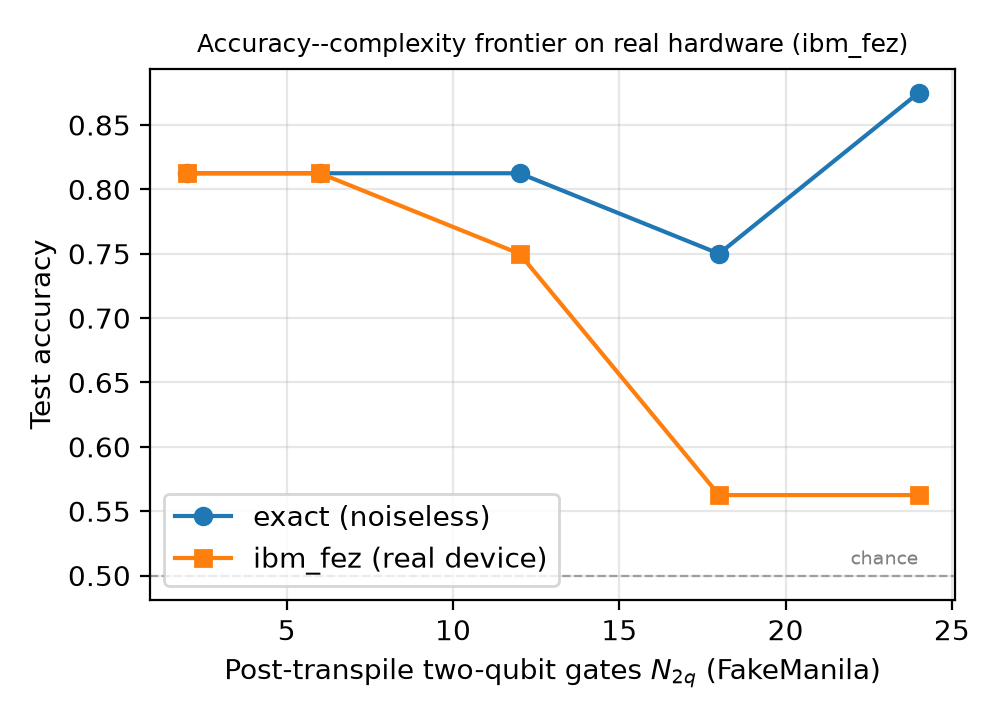
\includegraphics[width=0.80\columnwidth]{figures/fig_hardware_frontier.png}
\caption{Accuracy--complexity frontier on a physical IBM device (\texttt{ibm\_fez}, hard task).
In simulation accuracy is flat; on hardware it falls monotonically with $N_{2q}$, collapsing
toward chance for the full circuit. The widening gap is the cost of redundant entangling
capacity---and the case for compression.}
\label{fig:hw}
\end{figure}

\section{Conclusion}
Compressing a quantum Bayesian learner by greedy structured pruning reveals a clear capacity
boundary: most entangling structure is redundant---the learner sheds roughly two-thirds of its
two-qubit gates for free, and on the hardest task a compressed circuit beats the full one---yet
entanglement remains necessary, since removing it collapses the learner to chance. Structure
beats count, with learned masks outperforming random masks of equal budget. These conclusions
are not artifacts of simulation: on a physical IBM device the full circuit collapses to near
chance while the compressed circuit stays accurate. The result links cognitive capacity and
quantum-circuit capacity in one experiment, and shows that quantum models of cognition can
benefit from---not merely tolerate---the constraints of present-day hardware. Code and logs are
public.\footnote{\url{https://github.com/zoraizmohammad/qb-learner-compression}}

\begin{thebibliography}{00}
\bibitem{b1} T.~D. Ullman and J.~B. Tenenbaum, ``Bayesian models of conceptual development,'' \textit{Annu. Rev. Dev. Psychol.}, vol.~2, pp.~533--558, 2020.
\bibitem{b3} J.~R. Busemeyer and P.~D. Bruza, \textit{Quantum Models of Cognition and Decision}. Cambridge Univ. Press, 2012.
\bibitem{b4} A.~Kandala \textit{et al.}, ``Hardware-efficient variational quantum eigensolver for small molecules and quantum magnets,'' \textit{Nature}, vol.~549, pp.~242--246, 2017.
\bibitem{b5} L.~Leone \textit{et al.}, ``On the practical usefulness of the hardware efficient ansatz,'' \textit{Quantum}, vol.~8, p.~1395, 2024.
\bibitem{b6} M.~Cerezo \textit{et al.}, ``Variational quantum algorithms,'' \textit{Nat. Rev. Phys.}, vol.~3, pp.~625--644, 2021.
\bibitem{b7} J.~Preskill, ``Quantum computing in the NISQ era and beyond,'' \textit{Quantum}, vol.~2, p.~79, 2018.
\bibitem{b10} D.~Rodr\'iguez P\'erez \textit{et al.}, ``Error-divisible two-qubit gates,'' \textit{Phys. Rev. Applied}, vol.~19, p.~024043, 2023.
\bibitem{b16} Y.~Du \textit{et al.}, ``Quantum circuit architecture search for variational quantum algorithms,'' \textit{npj Quantum Inf.}, vol.~8, p.~62, 2022.
\bibitem{b19} E.~M. Pothos and N.~Chater, ``A simplicity principle in unsupervised human categorization,'' \textit{Cogn. Psychol.}, vol.~45, no.~1, pp.~45--85, 2002.
\bibitem{b24} H.~Abraham \textit{et al.}, ``Qiskit: An open-source framework for quantum computing,'' Zenodo, 2019.
\bibitem{b29} S.~Sim \textit{et al.}, ``Adaptive pruning-based optimization of parameterized quantum circuits,'' \textit{Quantum Sci. Technol.}, vol.~6, p.~025019, 2021.
\end{thebibliography}

\end{document}
